\chapter{Smart Contract and Distributed Ledger Technology}
With the development of technology, money transfers take place through networks, and we now need to update database entries that are governed by centralized institutions like banks. All of these procedures call for a third party to carry out the proper business dealings between unidentified parties. \\
Having third parties can lead to a number of issues, including the control of the entire transaction by a single authority and the invalidation of any transaction that accomplishes its goal. The new concept of a distributed ledger can be used to alleviate all of these problems. With this new technology, third parties are no longer necessary, and all transactions may be completed quickly between parties via a public network.\\
With the distributed ledger, it is impossible to alter transactions recorded in a ledger or identify the persons involved in these transactions \cite {Masood}. 
\section{Ledger} 
A ledger is a book or computer that keeps track of financial system transactions. There are two separate ledgers that look like this: \\
\textbf{Centralized Ledger} includes all recording of transactions involving firm resources, expenses, libraries, etc.\\
\textbf{Decentralized Ledger} is a database that shares data across the network. It allows transactions to be executed in public. Any participant at each node can have an identical copy of the ledger, which is already shared on the network.\\
If any change or update occurs on the ledger, each node constructs a new transition and votes using the consensus algorithm to choose the correct copy of the ledger. Once consensus has been reached, other nodes will be synchronized with the latest version of the ledger \cite{Ozsu}.

\section{Distributed Vs. Decentralized} 
Baran (1964) \cite{Baran} clarifies the distinction between decentralized and distributed. Decentralized refers to the absence of a central decision-making body. Every participant has the freedom to make their own decisions, and the system collects them all as subsequent behaviors. The process is divided among all participants in the distributed system, but there is no central authority; instead, decisions will be centralized. Decentralized databases are a collection of connected databases that operate autonomously in several locations, which is their fundamental distinction from distributed databases. \\
A distributed database, according to Ozsu et al. \cite{Ozsu}, is a group of various, logically connected databases that are dispersed throughout a computer network and provide transparent distribution to all users \cite{Ozsu}. 
According to this description, blockchain technology encompasses both kinds because it functions as a network and appears to users to be a single system. Blockchain is a type of distributed database system \cite{Ozsu}.


\section{Distributed Ledger Technology (DLT)} 
DLT refers to a database that offers participants identical copies of shared data that are updated using a sophisticated consensus mechanism. Costs are decreased, while transparency, traceability, and process speed are all improved. \\
There are various difficulties associated with this technology, some of which have not yet been solved. Scalability, separability, and data privacy are the three main issues with DLT \cite{Jose}. \\
\\
\textbf{How Does DLT Work?}\\
\\
DLT is the result of combining the main three technologies: \\
\hspace{1cm}\textit{-  P2P}: Each participant (node) functions both as a client and a server at the same time, using and contributing resources.\\
\hspace{1cm}\textit{- Cryptography} is used to authenticate the identity of the participant and the information between the two parties. Encryption helps in limiting access to information by other parties. \\
\hspace{1cm}\textit{- Consensus algorithm} allows network participants to come into agreement to add a new node (block) to the ledger \cite{Jose}.\\
\section{Blockchain}Blockchain is the most widely used distributed ledger, according to the World Bank Group \cite{Natarajan}, that stores and distributes data in units called "blocks." Each block's header includes details including a nonce, timestamp, block hash, and a hash pointer to the block before it. As a result, a digital chain is formed by connecting all of these pieces. \cite{Natarajan}. \\
Blockchain is described by Luke et al. \cite{Luke} as a collection of blocks that are connected to one another and encrypted. An identical copy of these records is kept locally on the PCs of network members. When a user requests a transaction, whether it be a transaction, a contract, or other information, the blockchain begins processing. \\
A P2P network of nodes broadcasts the transaction. Following then, the P2P network's nodes engage in a process known as verification in which they collectively check the transactions using hashes produced by an algorithm. Details of the transaction will be saved in a block after verification is finished. Finally, a new block is permanently and inevitably added to a chain \cite{Luke}.
The \textit{Genesis} block is the first block in the blockchain, and more nodes will be added to the chain once all nodes have reached consensus. The blockchain can expand without concern for information in the blocks being altered thanks to the consensus method. Since the blocks include transactions, the consensus procedure lasts for a set amount of time. When a transaction is added to a blockchain, there is a time lag between when the transaction was initiated and when it was added. Based on the block size, the number of transactions, and the consensus process, this confirmation time varies. There are several consensus mechanisms stated, including:
\begin{itemize}
    \item Proof of Work (PoW): 
    It is a system that promotes consensus without relying on a centralized authority. This method pits miners against one another to see who can enter their transactions into the blockchain first and earn incentives (such Bitcoin or Ether).\\
    Anyone who completes their assignment earlier can add their block first on the blockchain. Miners are participants in cryptocurrency transactions that connect to the blockchain and carry out tasks, validating transactions to add new blocks by solving a cryptographic challenge \cite{Pablo}.
    \item Proof of Stake (PoS): 
   It is a proof-of-work substitute that uses less CPU (Central Processing Unit) computation during mining. The likelihood of mining the following block in proof of stake relies on node balance. \\
    However, consensus procedures like proof of work are not necessary for private networks when users are acquainted. This specifically eliminates the requirement for mining and allows us access to a wider range of consensus procedures  \cite{Christidis}.
    \item Proof of Authority (PoA): It confirms accounts and allows them to add transactions in blocks. Compared to the previous approaches, this one is more vulnerable to attack because it is much more centralized and has higher transaction speeds \cite{Luke}.
    \item Practical Byzantine Fault Tolerance (PBFT): Byzantine Generals are some network users who communicate transaction-related information to others incoherently or fraudulently. Blockchain seeks to address this issue. \\
    This results in the unreliability of blockchain because there is no authority on it to rectify them. The PBFT algorithm leverages the idea of primary and secondary votes to try to reach a consensus in order to resolve this issue. If the primary vote is corrupted, the secondary vote can collectively change to a new primary after automatically evaluating the decisions made by the primary vote \cite{Luke}. 
\end{itemize}
Blockchain is associated with cryptocurrencies like Ethereum, Bitcoin, Litecoin, etc. Gupta (2017) \cite{Gupta} identified five core attributes through which blockchain builds trust:
\begin{itemize}
    \item Distributed ledger: No single authority has control over the data. It is distributed and updated throughout the network, and any new changes are distributed to all users.
    \item Organized and adaptable: Because smart contracts can be carried out on the blockchain, the technology may be developed to support company operations.
   \item Transparent and auditable: Since everyone has access to the same ledger, can confirm transactions, and can determine the owner, there is no need for a third party or other authority. 
    \item Secure, private, and indelible:
    Blockchain offers these advantages by making use of tools like cryptography and permissions, which make sure that unauthorized users can't access the network. It indicates that participants are who they say they are.
    \item Consensus: To validate the transition, all nodes on the network must concur, and the blockchain implements this process via a consensus mechanism \cite{Gupta}.
\end{itemize}
\\
\textbf{Type of Blockchain}
Blockchain is used to transmit information across a secure network, according to Aithal et al. \cite{Aithal}. Public and private networks were the two main types of blockchain technology. Blockchain technology can alternatively be categorized as consortium blockchain technology or hybrid blockchain technology, according to further investigation \cite{Aithal}. \\
All blockchains, it should be mentioned, are node-based and run on P2P (peer-to-peer) networks. According to Aithal et al. \cite{Aithal}, there are three different kinds of blockchain: consortium blockchain, private blockchain, and public blockchain. The hybrid blockchain is an additional type of blockchain that exists \cite{Aithal}.
\begin{itemize}
    \item \textbf{Public Blockchain} is the main variety of blockchain that is open and decentralized by nature. Anyone is allowed to join the network and establish consensus in this system. Any miner (participant) on a public blockchain can develop consensus techniques like proof of work and proof of stake to validate transactions with a low validity rate \cite{Kalra}.
    \item \textbf{Private Blockchain} is not open and restricted in this way that Only authorized participants have the ability to validate transactions. As a result, it offers improved privacy, enhances scalability, and reduces security concerns. All participants in this network are known, hence there are no mining computations necessary for this blockchain to establish a consensus \cite{Kalra}. 
    \item \textbf{Consortium Blockchain} is a semi-decentralized blockchain that is used to carry out operations for just one company, such as a bank, etc. A consortium blockchain differs from a private blockchain in that it is managed by multiple parties rather than just one \cite{Aithal}.
    \item \textbf{Hybrid Blockchain} is a combination of private and public blockchain. As a result, it combines the advantages of a private blockchain's privacy with the security and openness of a public blockchain. \\
    The user of this kind of blockchain can regulate who has access to what data on the blockchain. On a private network, a transaction can be validated before the user releases it to the public blockchain. By doing this, only a portion of the records can be made public while the remainder can be kept secret on a network \cite{Aithal}.
\end{itemize}

\section{Ethereum}
Currently, Ethereum is the world's most active public blockchain. It is a different cryptocurrency that is based on the blockchain and is comparable to Bitcoin. The transactions are published by the users on the network, which uses a consensus mechanism to store them in blocks and add them to the blockchain. In Ethereum, "state" refers to the current status of the various accounts that make up the blockchain. In Ethereum, a user's account may either be an unrelated external account or a contract account that receives ongoing blockchain storage. \textit{Ether} serves as the system's virtual money. By establishing a new contract or triggering an already-existing contract, the transaction has the ability to alter the system's state \cite{Ilya}.
\section{How Does Ethereum Work?}
In this subsection, we will focus on the Ethereum workflow at a technical level.
\subsection{Blockchain}
The blockchain contains some information that we have utilized in our project. Therefore, we focus on it more, as follows:
\begin{center}
	\begin{figure}[htb!]
		
		\begin{minipage}{0.5\linewidth}
			\centering
			\includegraphics[width=1.95\textwidth]{images/chap01_Blockchain.png}
		\end{minipage}
		\caption[Block contents]{Block contents \footnote{https://archive.researchworld.com/three-ways-that-blockchain-can-improve-the-quality-of-market-research/}}
		
	\end{figure}
	
\end{center}
\begin{itemize}
   \item \textbf{Block} as a data structure within the blockchain, contains different functions, which include transaction hashes and some other additional information for blockchain technology. following information was described by Gavin Wood et al. \cite{Gavin} and we used it in our project: \\
    \begin{itemize}
        \item \textit{parentHash} is the hash of the parent block's header.
        \item \textit{stateRoot} is the hash of the root node of the state after execution of all transactions is applied.
        \item \textit{transactionRoot} is the hash of the root node of data populated with a transaction in the transactions list inside the block.
        \item \textit{receiptRoot} is the hash of the root node of the data populated with the receipts of transactions in the block.
        \item \textit{logsBloom} composed of log information.
        \item \textit{difficulty} represents the difficulty level of the block.
        \item \textit{number} is the number of ancestor blocks.
        \item \textit{gasLimit} represents the current limit of gas in the block.
        \item \textit{gasUsed} is the amount of gas used for the transaction in the block.
        \item \textit{timestamp} is the time of reasonable output.
        \item \textit{extraData} is a byte array containing relevant information in the block.
        \item \textit{nonce} is the number of several computations that have been done in the block.
    \end{itemize}
    \item \textbf{Mining} is a process of computation on the blockchain to verify and add a block. A new block is added by the miner, and then it is verified by others. Anyone can join the mining pool, however, the likelihood of discovering a valid block relies on the computer's processing capability. A miner may occasionally discover an uncle block. "An uncle block" is a legal block that is eventually surpassed by a faster block. A hash will be added to a valid block, and an Uncle block is rewarded with $\frac{7}{8}$ of the total block value. A valid block may have up to two uncle blocks added to it, and each uncle block earns the valid block's miner an additional $\frac{1}{32}$ worth of ether \cite{Egbertsen}.
\end{itemize}
\subsection{Ether}
It serves as both Ethereum's fuel and a means of payment. In order to successfully mine (find the solution and add blocks), you need five ethers. It becomes less ether, such as 4.375 ether, and becomes an uncle block if the miner finds a solution but does not act quickly enough. There can only be two uncle blocks per block, and each uncle block is paid $\frac{1}{32}$. If a second miner also discovers the answer, the block cannot be added to the blockchain, and the first miner only gets a reward of a couple of ether \cite{Egbertsen}.
\subsection{Account}
There are two types of accounts in Ethereum:\\
- \textit{Normal account} is controlled by the private key. The owner of this account can send either a message.\\
- \textit{Contract} account is controlled by code. It can only fire a transaction in response to other transactions \cite{Egbertsen}. An account encompasses four fields:\\
 \begin{itemize}
    \item \textit{Nonce} is the number of transactions sent from this address \cite{Gavin}.
    \item \textit{Balance} is the number of Wei owned by this address \cite{Gavin}.
    \item \textit{StorageRoot} is the hash of the root node of the Merkle Patricia tree, which encodes the content of an account. It should also be noted that the Merkle tree is used for data representation in the block header \cite{Gavin}.
    \item \textit{CodeHash} is the hash associated with this account that would be executed when this account address receives a message call and would no longer be changeable. For later retrieval, all information pertaining to this account is kept in the database under the associated hash code \cite{Gavin}.
\end{itemize}
\textbf{Hash Function}
At the National Institute of Standards and Technology (NIST), the SHA3 standardization procedure was finished in August 2015. The Secure Hash Algorithm-3 (SHA-3) family of functions for binary data is described by this standard. The \textit{Kacak} algorithm, also known as NIST and the winner of the SHA3 cryptographic hash algorithm competition, serves as the foundation for each hash function. There are four functions in the SHA3 family, each having a distinct length of 224, 256, 384, or 512 bits.
The input to the hash function is referred to as a \textit{message}, and the output is referred to as a \textit{hash value}, where the message's length might vary but the hash value's length is always constant \cite{Dworkin}.


\begin{center}
	\begin{figure}[htb!]
		
		\begin{minipage}{0.2\linewidth}
			\centering
			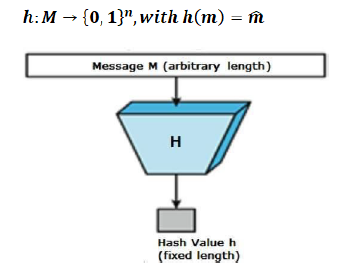
\includegraphics[width=4.5\textwidth]{images/chap01_hash_function.png}
		\end{minipage}
		\caption[Image of hash function]{Image of hash function \cite{Dworkin}}
		
	\end{figure}
	
\end{center}

On the Ethereum network, gas is the fuel that must be purchased prior to completing a transaction. The consumed gas will not be refunded if the transaction is rolled back \cite{Egbertsen}.\\
\textbf{Transaction}
 A transaction is a cryptography-signed instruction that is carried out by an external actor, which can be a person or another contract, according to Gavin Wood et al. \cite{Gavin}. The transaction describes these fields:
     \begin{itemize}
         \item \textit{Nonce} is the number of transactions sent by the sender.
         \item \textit{GasPrice} is the number of wei to be paid per unit of gas.
         \item \textit{GasLimit} is the amount of gas that can be used for transactions.
         \item \textit{To} is the address to which that contract sends a transaction.
         \item \textit{Value} is the number of wei that is transferred in the transaction.
    \end{itemize}
\textbf{Message} is sent by a contract and has the same attributes as a transaction, but $gasPrice$ is not included \cite{Egbertsen}.\\
\subsection{Contract}
It is an Ethereum blockchain account that is managed by code and has its own code. Every time a message is received, the contract's internal code is activated, enabling it to read and write contract storage or send messages.\\
A contract in Ethereum is an autonomous agent that executes when it receives a message or transaction and has control over its balance and the key/value stored as constant variables. This means that the contract is an autonomous agent that carries out some operations that are programmed to achieve the user's goals. \\
The contract's long-lasting keys and values are used when the contract begins to function \cite{Egbertsen}.

\subsection{Smart Contract}
Nick Szabo \cite{Szabo} first popularized the phrase "smart contract" in 1994 after realizing that DLT might also be used for them. \\
The definition of a smart contract is given by Nick Szabo \footnote{https://www.fon.hum.uva.nl/rob/Courses/InformationInSpeech/CDROM/Literature-\break /LOTwinterschool2006/szabo.best.vwh.net/smart.contracts.html}: \textit{Smart contract is a computerized transaction protocol that executes the terms of a contract}. He had an idea for how to design contracts that automatically and effectively enforce the terms between the parties to a transaction. \\
Each node executes a smart contract as part of the block-building process. When a transaction occurs on the blockchain, a block is created.
Each smart contract has its own address, which is an essential component. A node can construct a specific transaction by giving it a contract address and carrying the contract code, which makes it possible for this transaction to execute the contract code at the time of formation.
The address won't ever change after that because the contract will become a permanent part of the block. A message should be sent to the contract's address that contains the method and input data whenever a node wants to invoke a method inside the contract. \\
When a new block is created, the contract will execute as part of that process and then either return value or store data on the blockchain \cite{Payrott}.\\
\\
\textbf{Solidity} is a high-level, Turing-complete language with a syntax resembling JavaScript. The contract is comparable to classes in object-oriented programming languages, which have fields for persistently storing contracts and methods that both internal and external transactions can call. Either a new instance of this contract must be created or a transaction must be made to a known contract address in order to interact with another contract.\\
Solidity, in theory, offers certain fundamentals for getting at blocks and transaction information, such as \textit{msg.sender} for getting at an account's address or \textit{msg.value} for getting at the amount of \textit{wei} transmitted by the transaction. Additionally, it employs several features, such as \textit{call} and \textit{send} to transfer money to another contract. These functions are used to transfer value and translate it into internal calls to transactions, which cause the contract to run code in addition to transferring value or may fail to run owing to a lack of gas \cite{Ilya}.